% =================================================

\begin{frame}
\frametitle{Protocol}
\framesubtitle{Protocolls used in different cities}
\begin{figure}
\centering
\missingfigure[figwidth=7cm]{}
\caption{Missing figure caption}
\end{figure}
\end{frame}

% =================================================

\begin{frame}
\frametitle{Data sources}
\framesubtitle{Overview of traffic light control (Ampelbeeinflussung)}
\begin{figure}
\centering
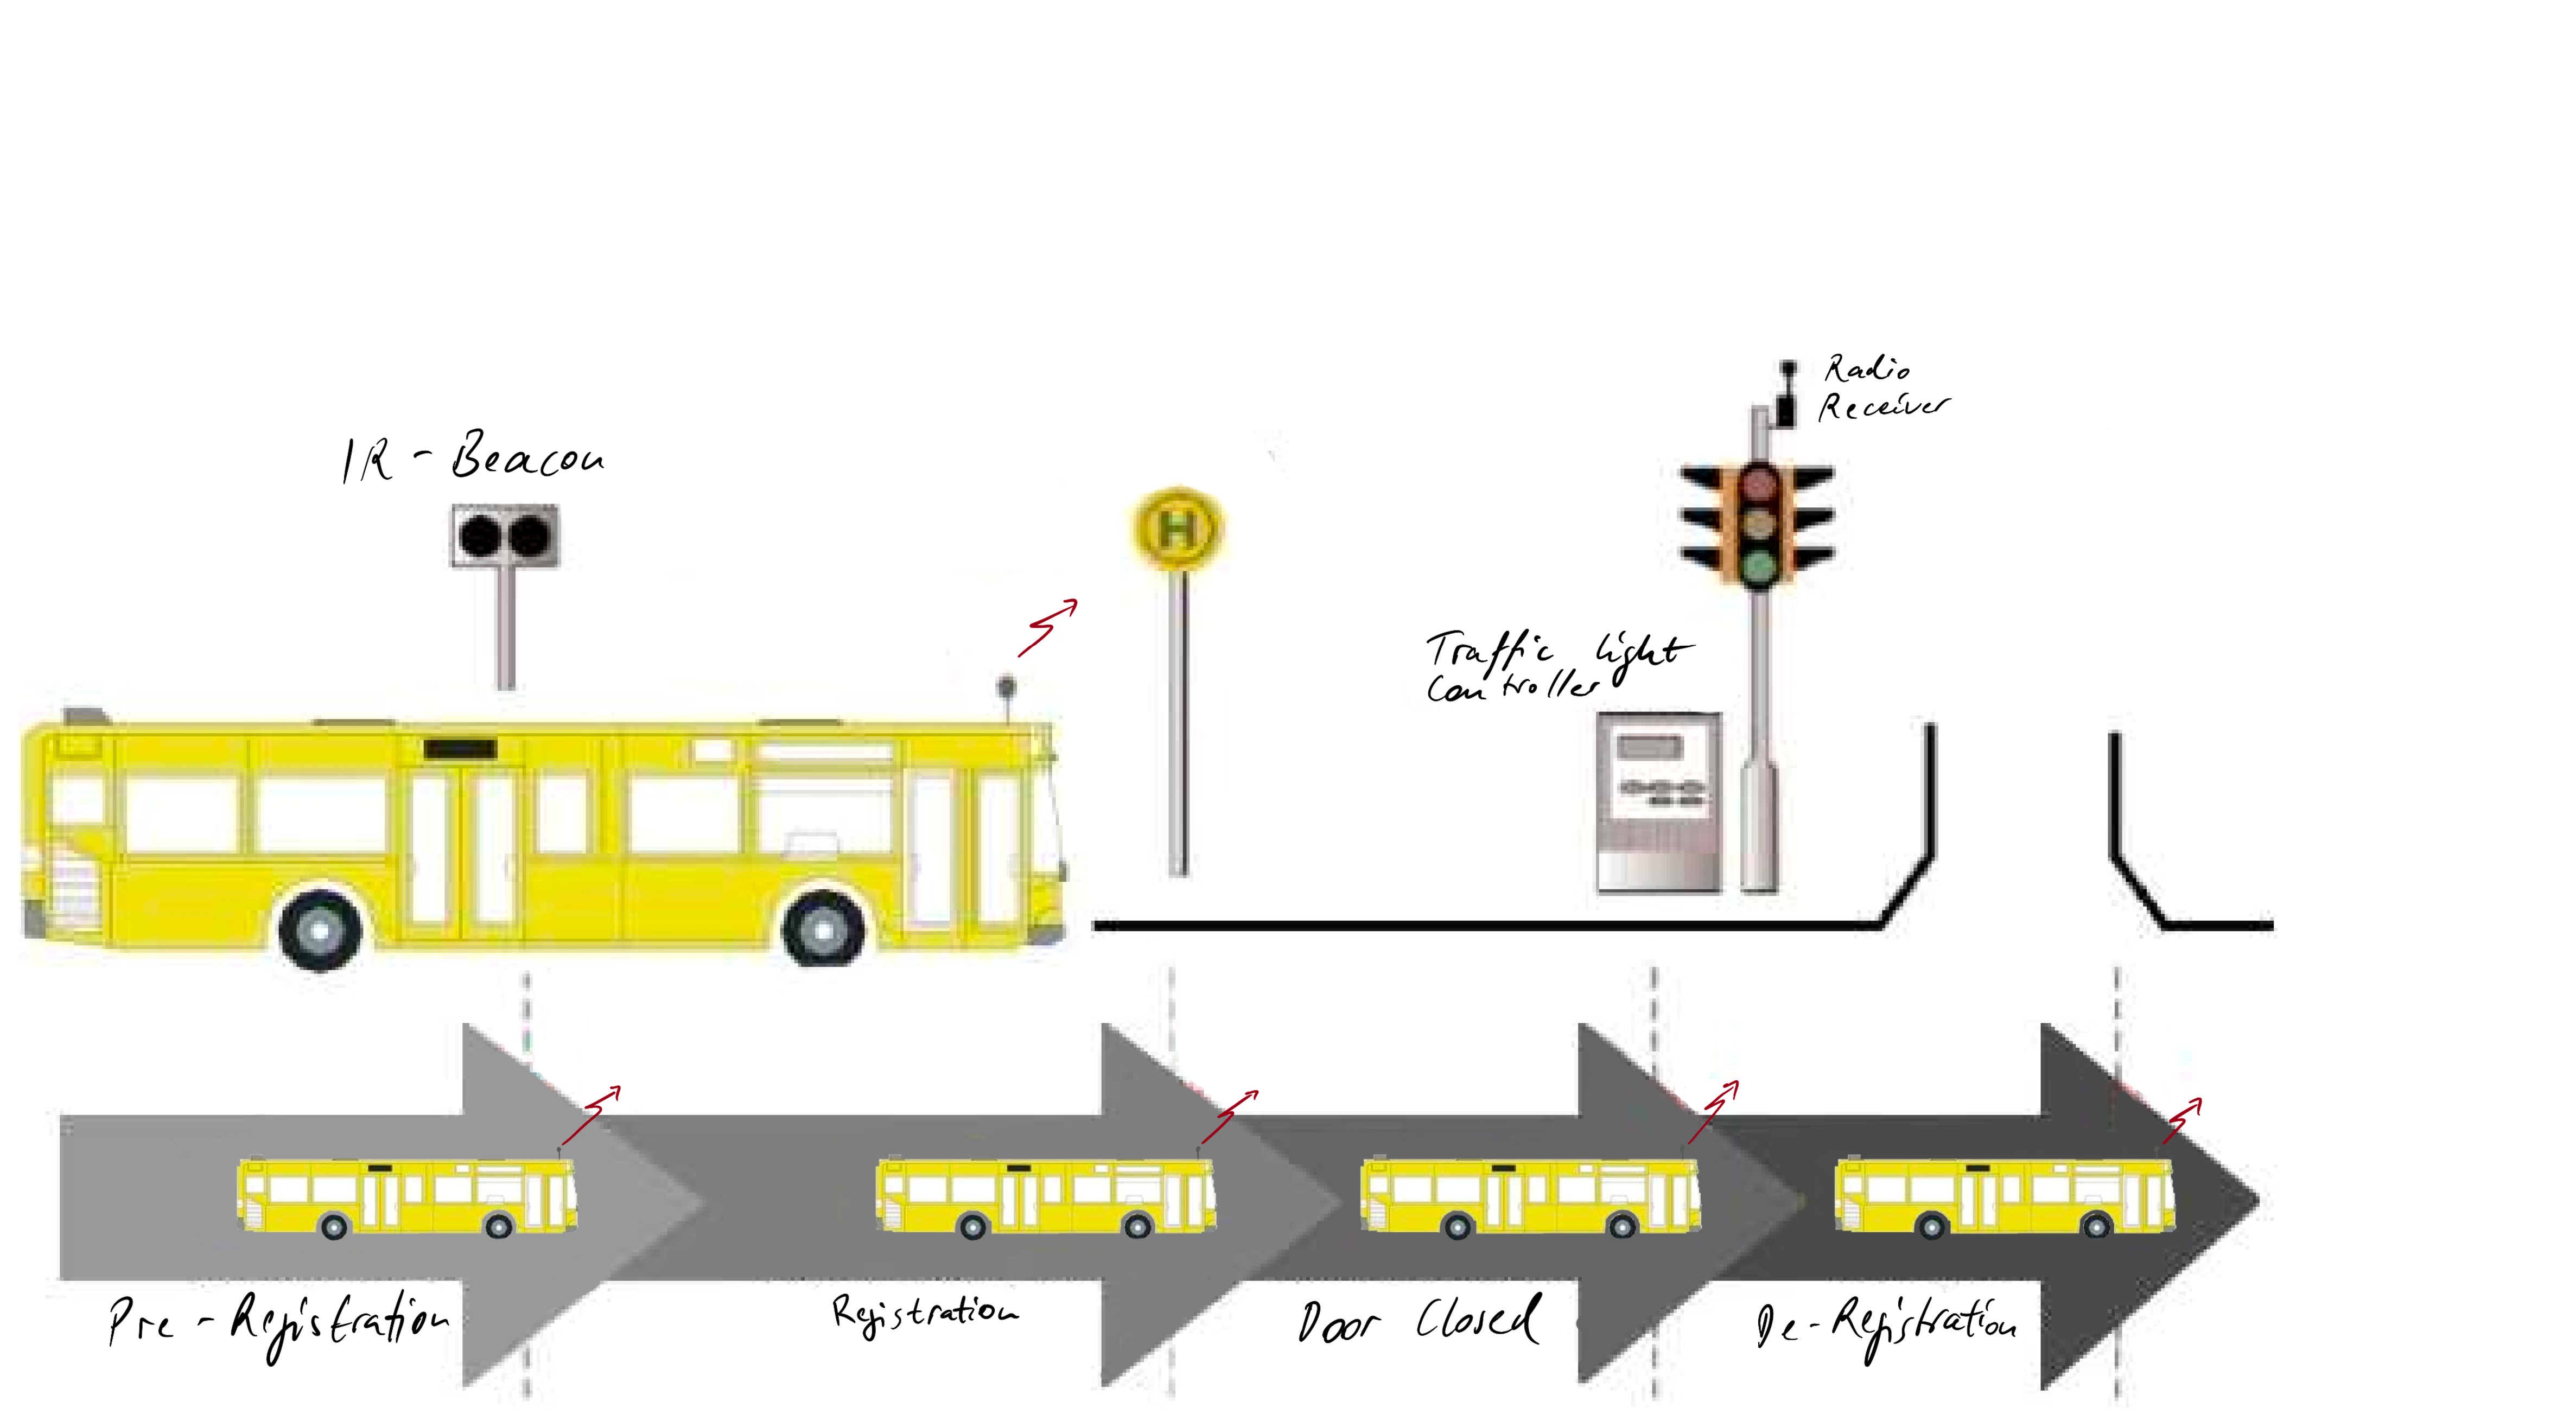
\includegraphics[height=0.65\textheight]{figs/lsa-beeinflussungs-stecke.pdf}
\caption{Traffic light controlled by radio link of busses and trams}
\end{figure}
\end{frame}

% =================================================

\begin{frame}
\frametitle{Data sources}
\framesubtitle{Overview of traffic light control (Ampelbeeinflussung)}
\begin{figure}
\centering
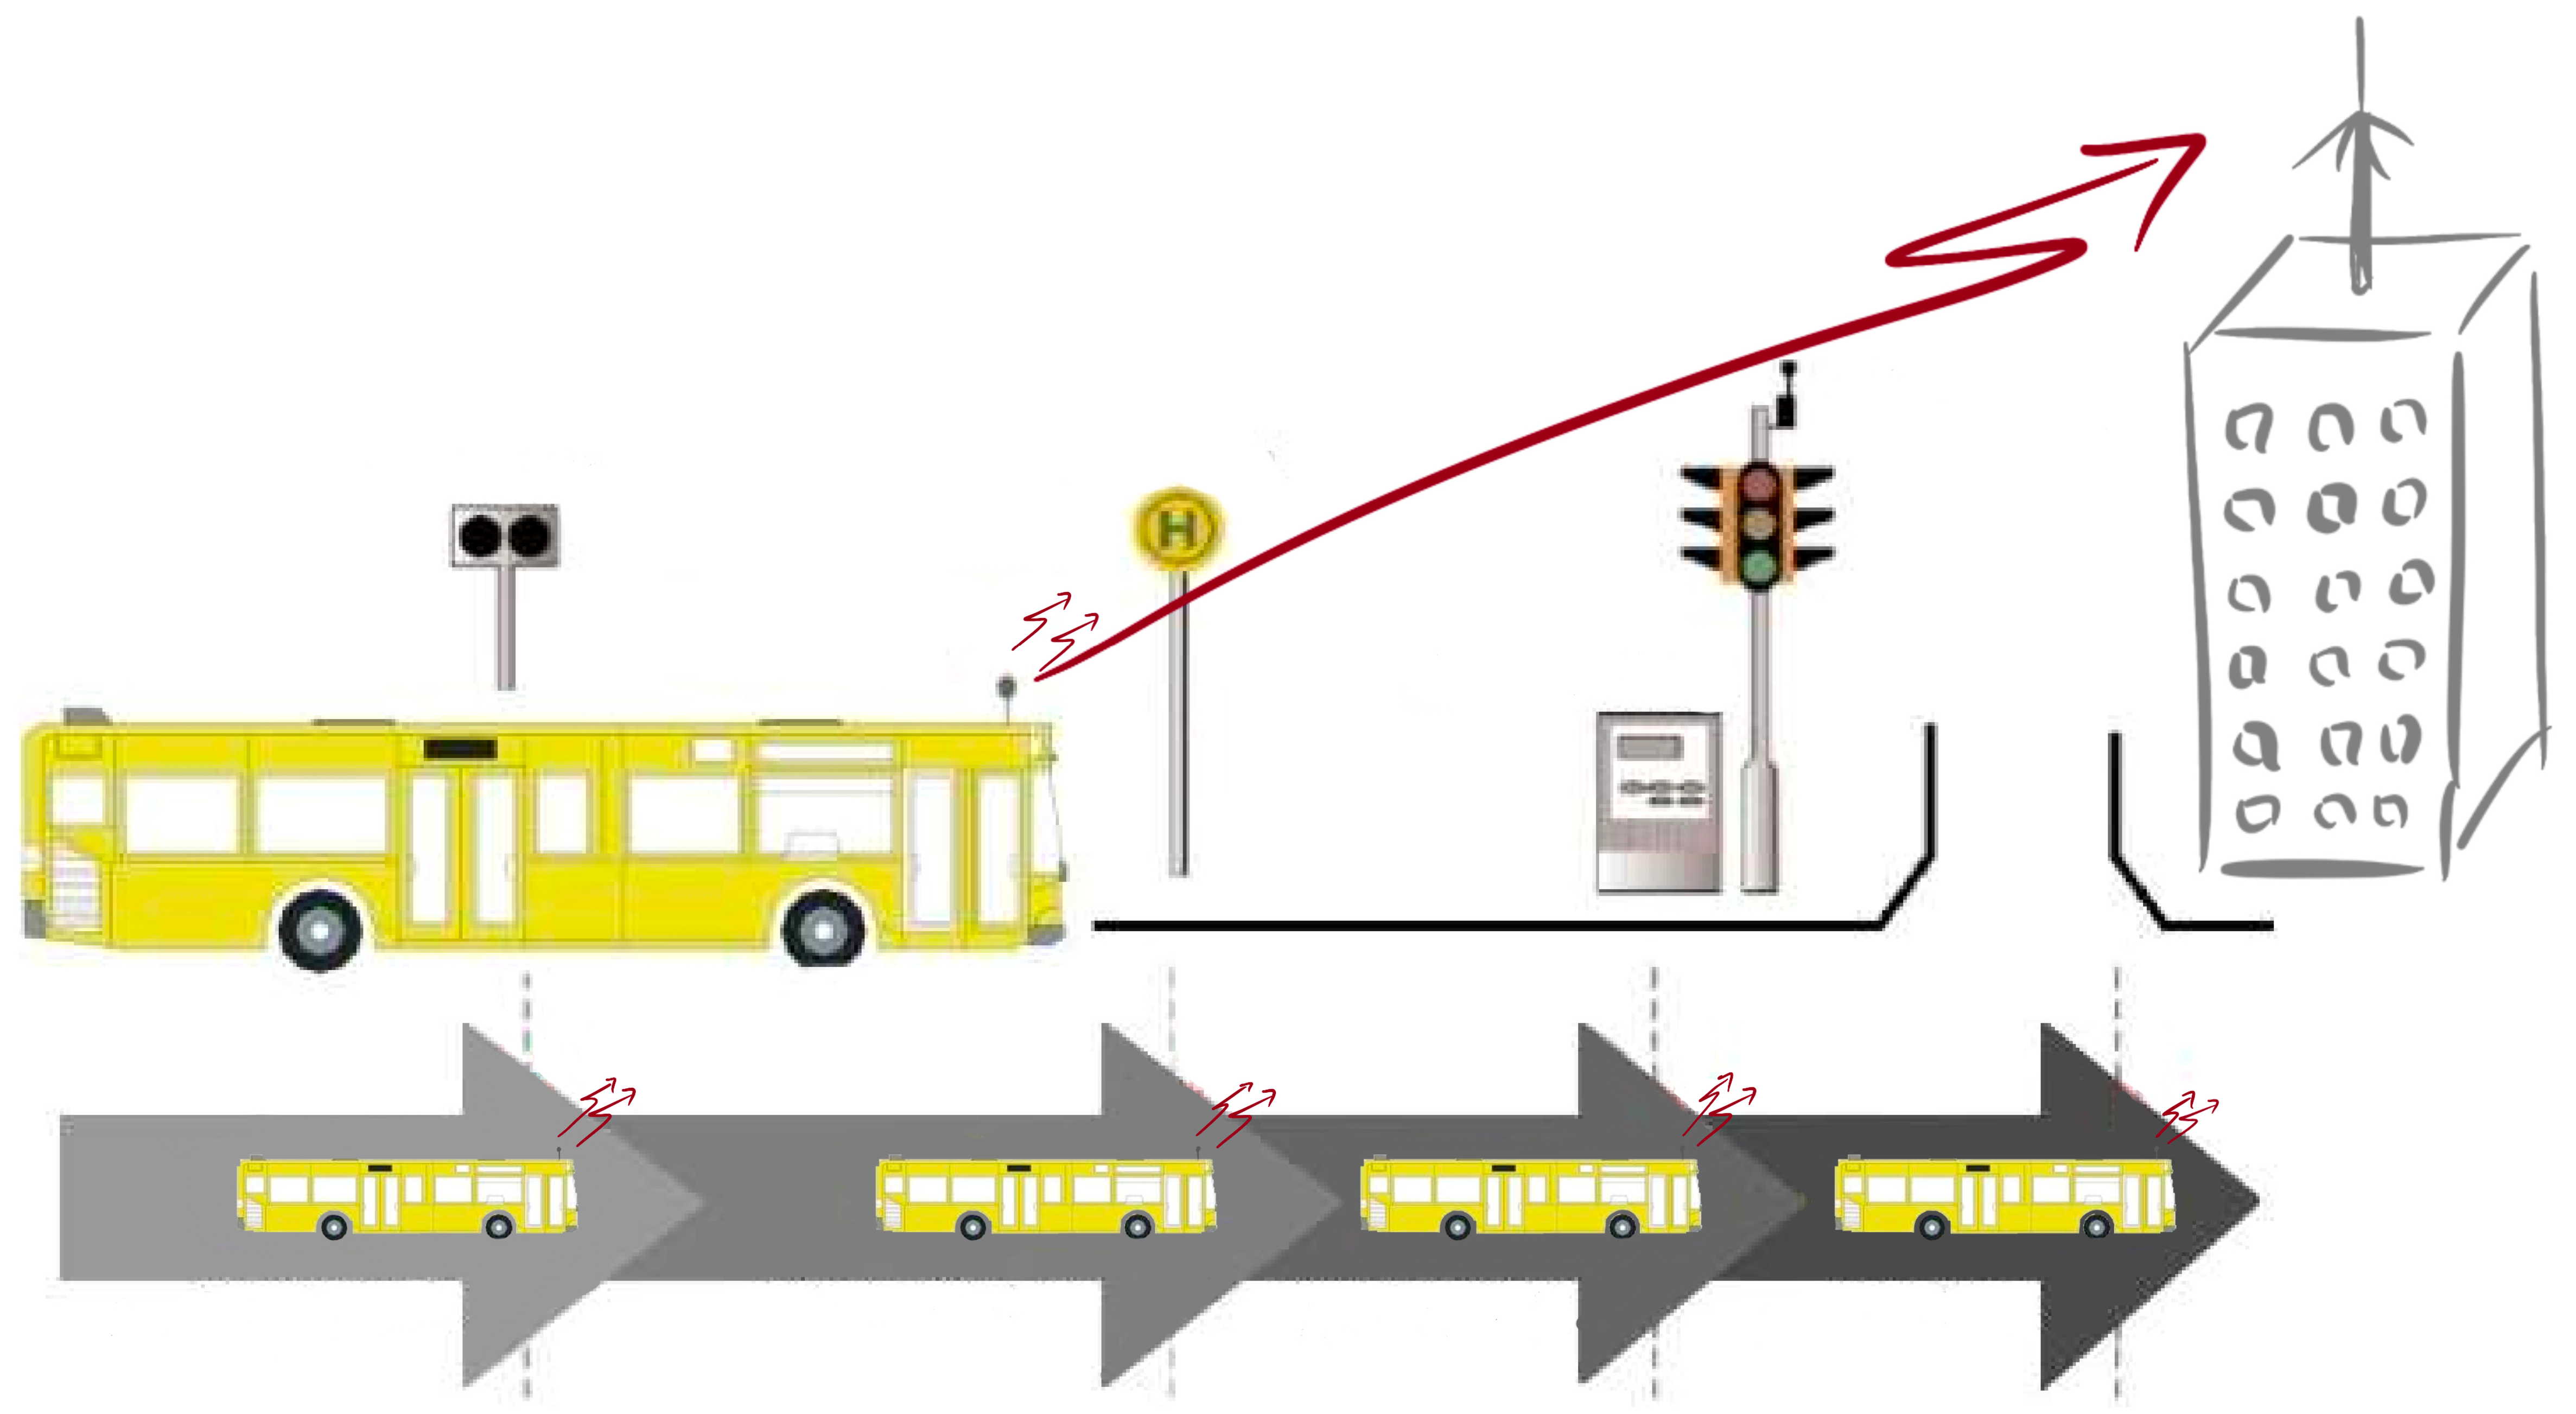
\includegraphics[height=0.65\textheight]{figs/lsa-beeinflussungs-stecke-mit-antenne.pdf}
\caption{Radio signals can be received by our antennas}
\end{figure}
\end{frame}

% =================================================

\begin{frame}
\frametitle{Data sources}
\framesubtitle{Receiver overview}
\begin{figure}
\centering
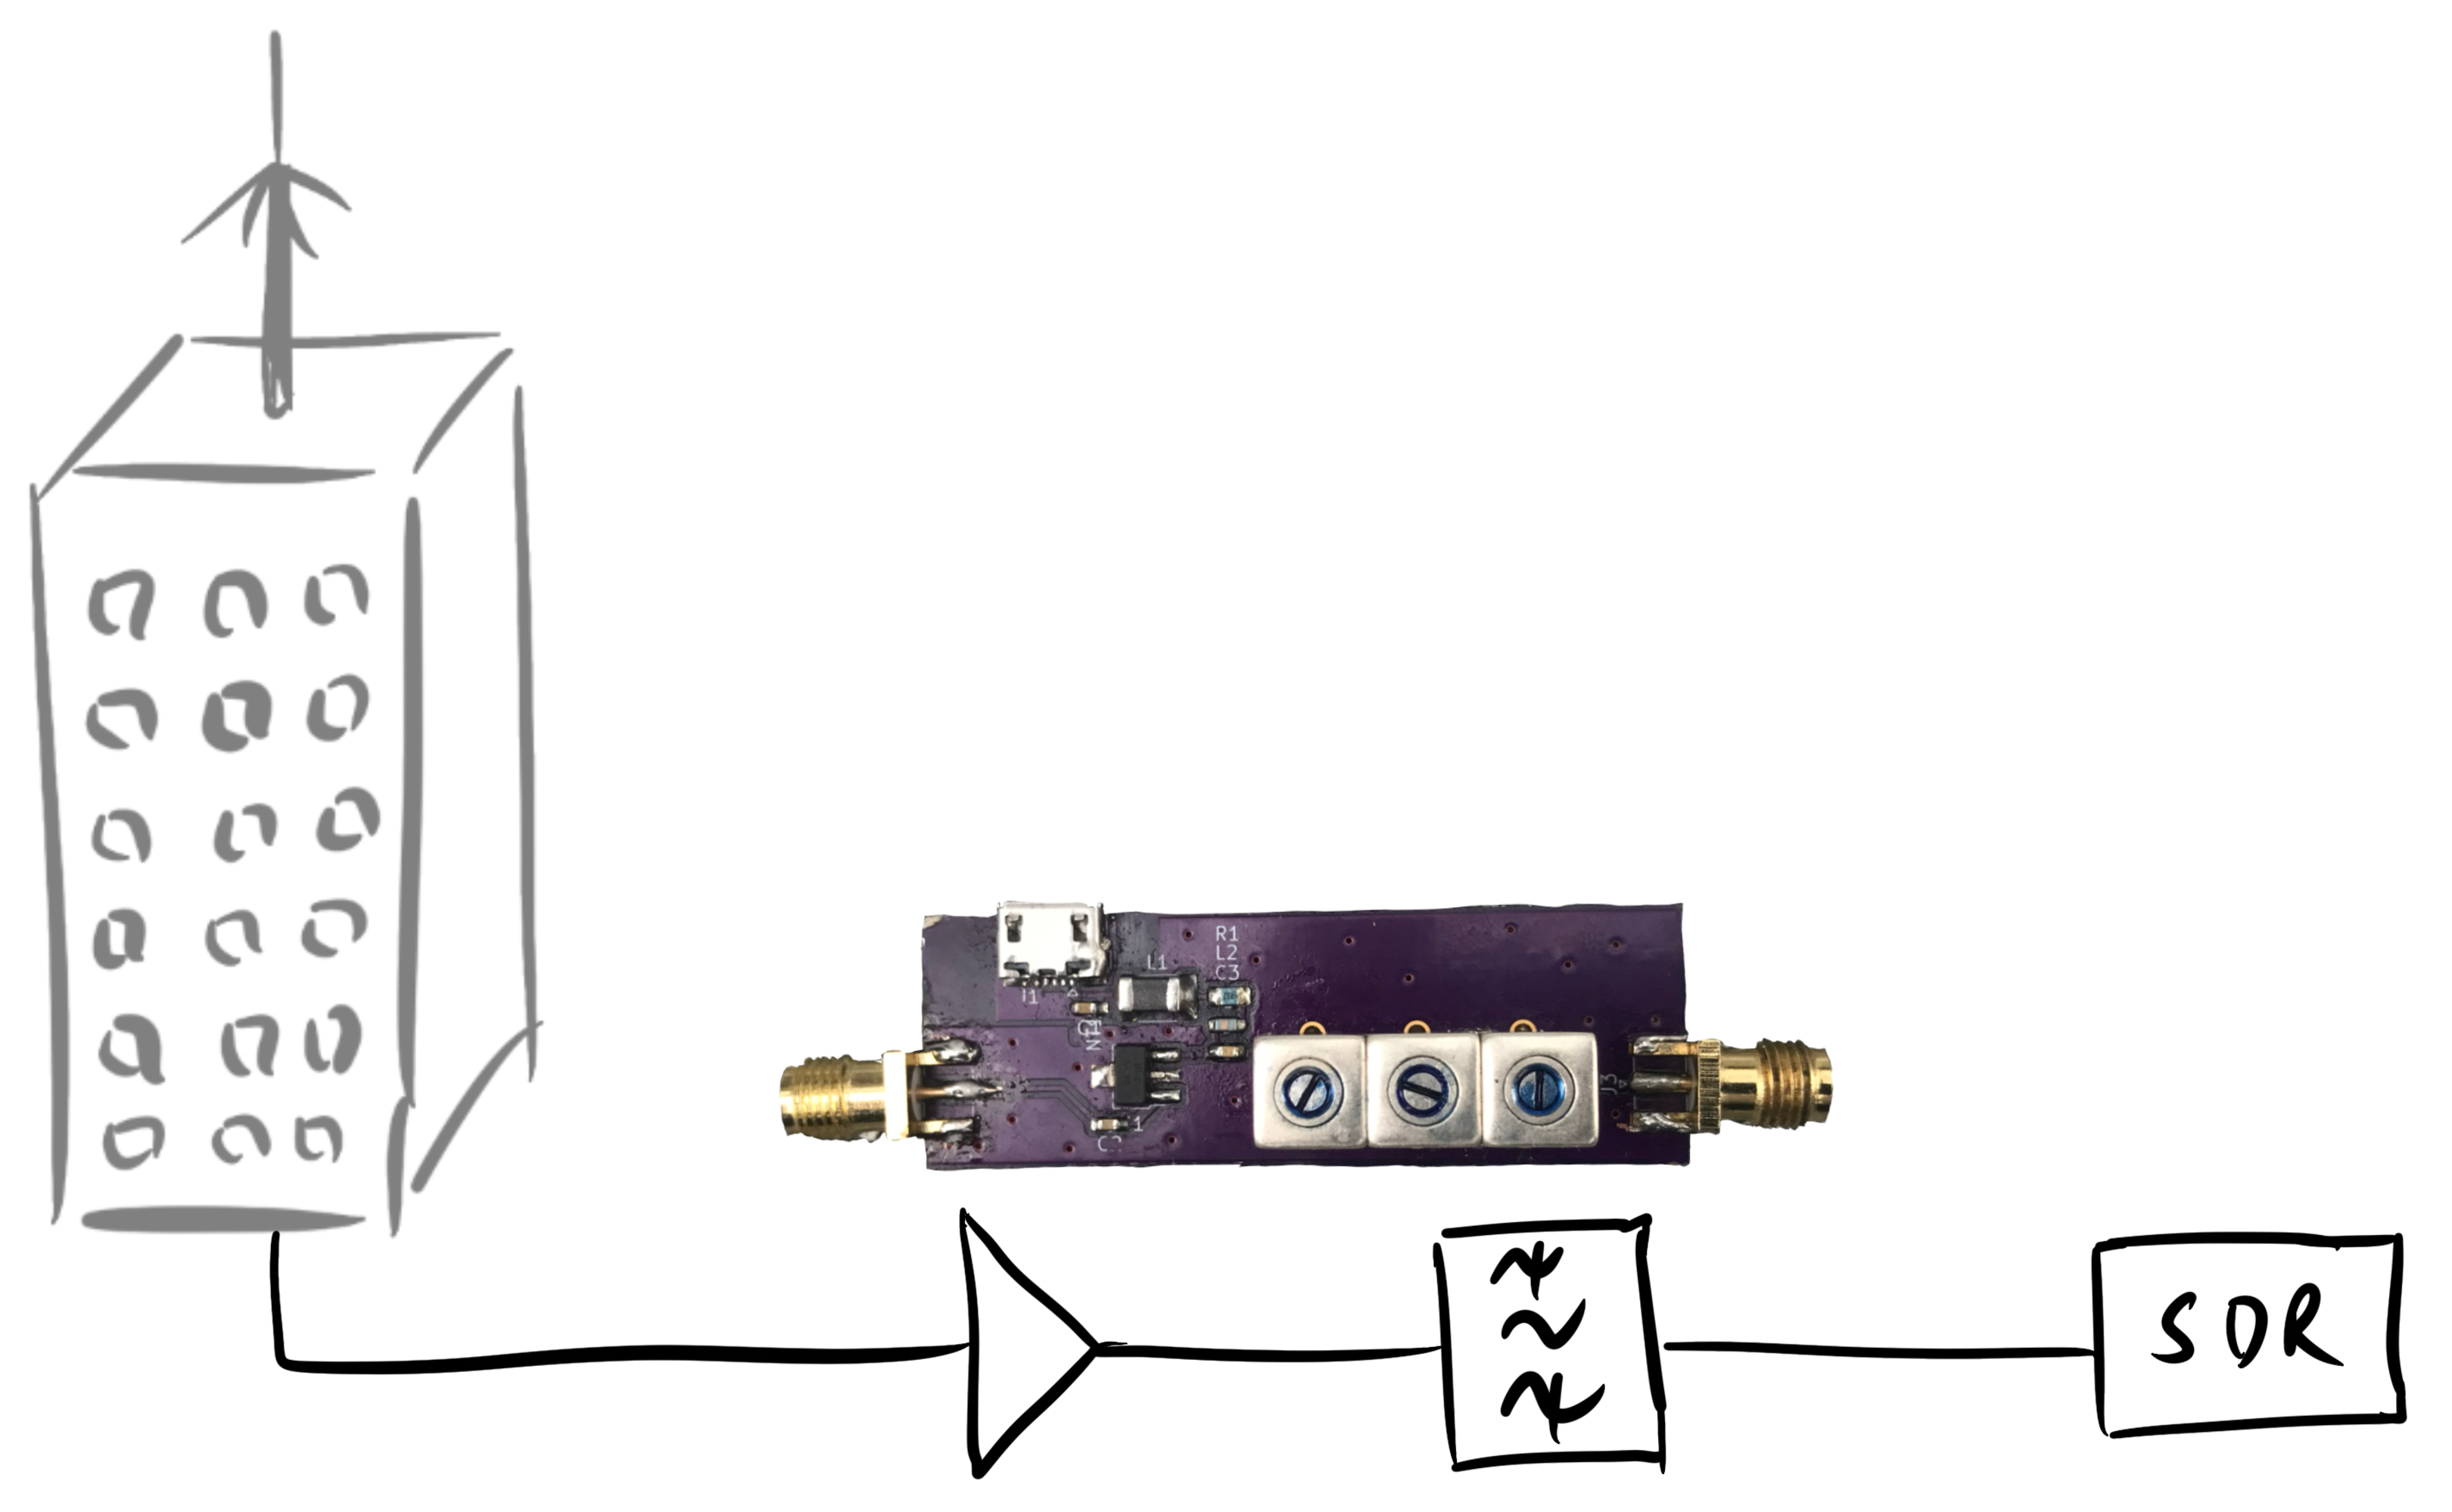
\includegraphics[height=0.65\textheight]{figs/antenna-filter.pdf}
\caption{Schematic overview of the receiver hardware}
\end{figure}
\end{frame}

% =================================================

\begin{frame}
\frametitle{Protocol}
\framesubtitle{VDV 420}
	\begin{itemize}
		\item which protocol?
		\item which frequency?
		\item some background on Ampelbeeinflussung and VDV 420 / 426
		\item R09 telegrams of trams and busses standardized in \href{https://knowhow.vdv.de/documents/420/}{VDV 420}
	\end{itemize}
\end{frame}

% =================================================

\begin{frame}
\frametitle{Protocol}
\framesubtitle{VDV 420 data}
\begin{itemize}
	\item what data can we receive?
	\begin{itemize}
		\item Tram identification data: line number, run number, destination number
		\item Location data: traffic light id, direction, registration\_type
		\item and some other (delay)
	\end{itemize}
\end{itemize}
\end{frame}

% =================================================

\begin{frame}
\frametitle{Protocol}
\framesubtitle{VDV 420 physical layer}
\begin{itemize}
	\item Minimum Shift Keying with \SI{2400}{Baud}
	\item bursty packet transmittion
		\item what frequency?
		\begin{itemize}
			\item look at the range of frequencies of RBL380, TODO add ranges
			\item take a look at our table, TODO link
			\item osint
		\end{itemize}
\end{itemize}
\end{frame}

% =================================================

\begin{frame}
\frametitle{Protocol}
\framesubtitle{Frequency identification}
\begin{figure}
\centering
\missingfigure[figwidth=7cm]{}
\caption{Screenshot of the bursty transmittion pattern}
\end{figure}
\end{frame}

% =================================================

\begin{frame}
\frametitle{Protocol}
\framesubtitle{Physical layer used in different cities}
\begin{figure}
% https://opus4.hbz-nrw.de/opus45-bast/frontdoor/deliver/index/docId/2595/file/V353+BF+Gesamtversion.pdf
% page 25
\begin{columns}
\column{.5\linewidth}
\centering
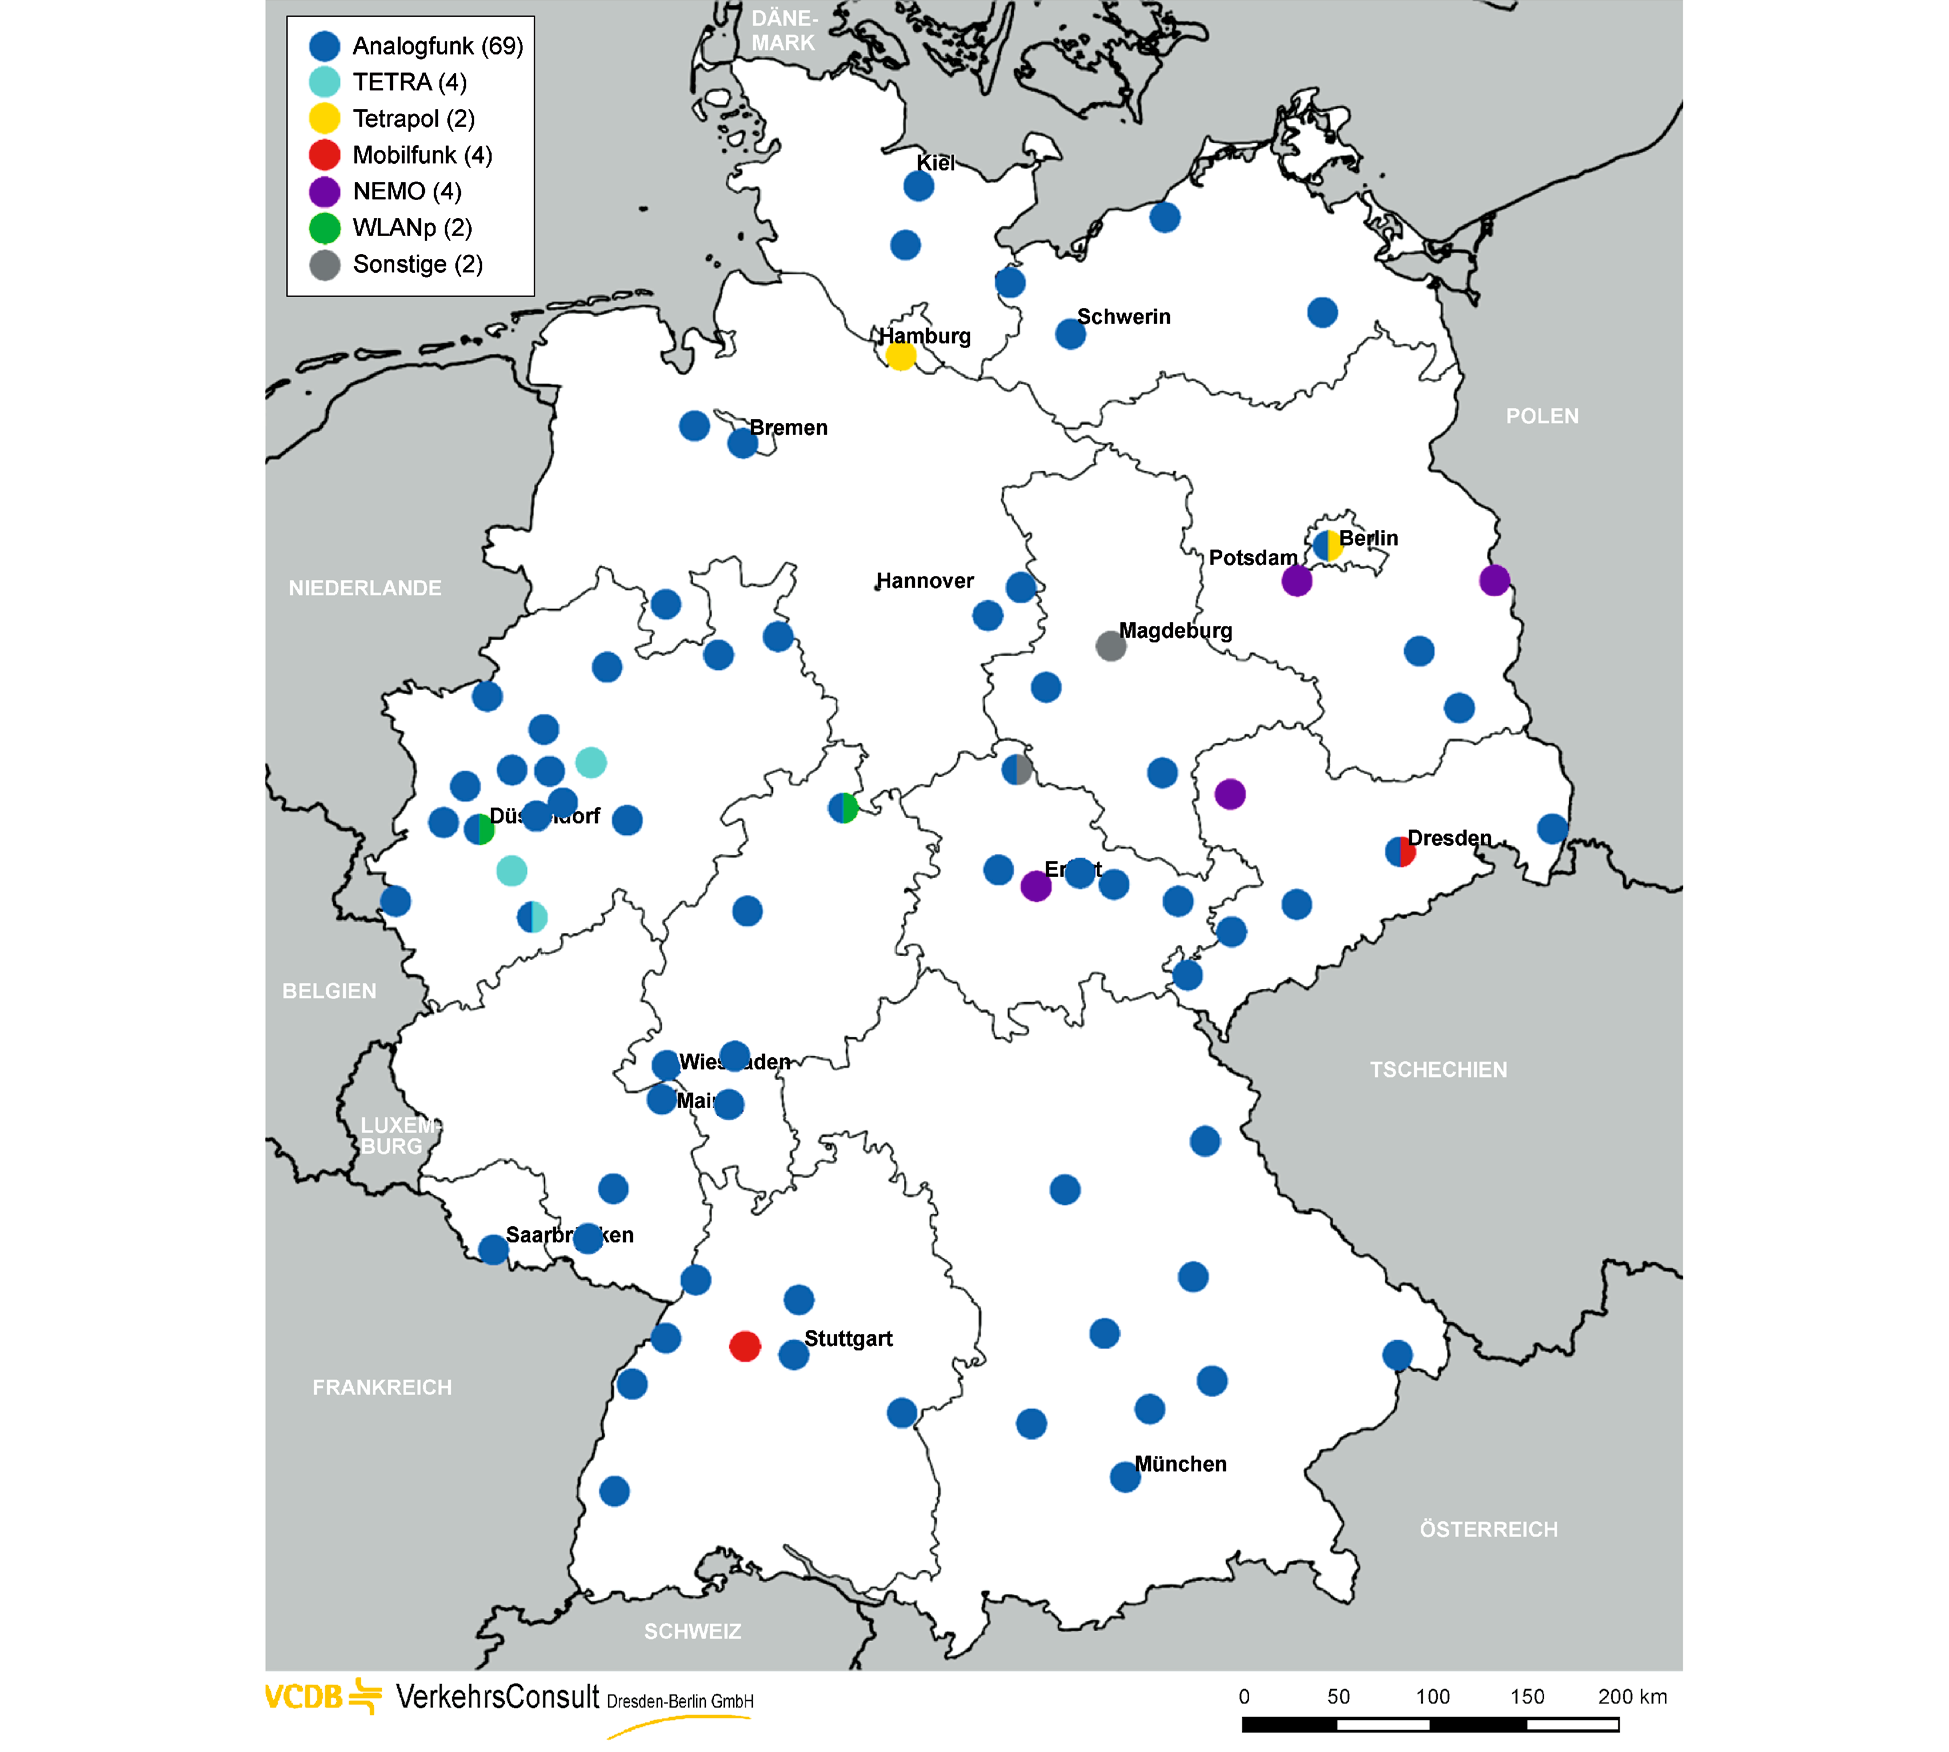
\includegraphics[height=0.8\textheight]{figs/vcdb-map-ampelbeeinflussung.png}
\column{.5\linewidth}
\caption{Map with selected locations which have traffic lights, controlled by public transport. Blue points use the standard we implemented.}
\vspace{0.5cm}
\begin{itemize}
	\item different physical layer protocols described in VDV 426
\end{itemize}
\end{columns}
\end{figure}
\end{frame}

% =================================================
